\newpage
\section*{Comparison of First Tries}
This is a small collection of plots showing the first few ideas and comparing the initial performance. 

\begin{figure}[H]
    \centering
    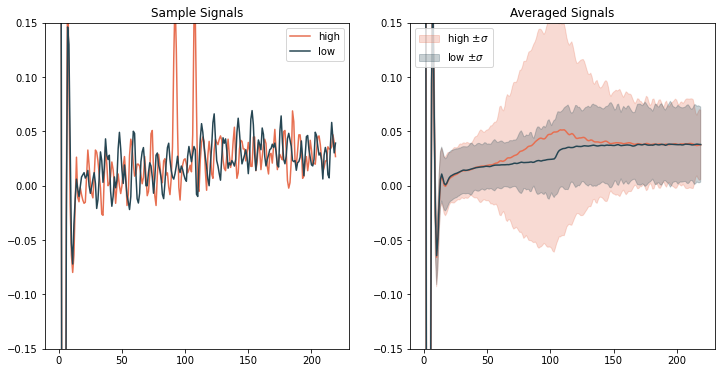
\includegraphics[width = \textwidth]{Figures/johann_first/sample.png}
    \caption{Comparison of the high and low pass signals. The left is an example of two read-outs (one high and one low respectively), while the right shows the averaged signals over the training set, the standard deviations are plotted as well.}
    \label{fig:samples}
\end{figure}



\begin{figure}
    \centering
    \includegraphics{FFT TRANSFORMED COMPARISON}
    \caption{Similar to Fig. \ref{fig:samples} but in a Fourier transformed space. Absolute value of frequencies are taken. The x-axis is just index and can be ignored. }
    \label{fig:samples_fft}
\end{figure}

\begin{figure}
    \centering
    \includegraphics{AUC}
    \caption{Comparison of the ROC curves for the different metods listed.}
    \label{fig:AUC_comparison}
\end{figure}

\begin{table}[]
\caption{A comparison of the test-metrics for different methods, we tried in the classification process.}
\label{tab:Metric Comparison}
\begin{tabular}{lll}
Name                 & Accuracay & AUC   \\
1D_conv              & 0.855     & 0.906 \\
feed_forward_network & 0.796     & 0.87  \\
LSTM                 & 0.858     & 0.912 \\
peak_height_adjusted & 0.836     & 0.875 \\
TCN                  & 0.798     & 0.891 \\
umap_fft             & 0.804     & 0.867 \\
umap_real_time       & 0.746     & 0.805 \\
xgb_real_time        & 0.821     & 0.875
\end{tabular}
\end{table}